\section{The Seven Miracles as an Esoteric School}

\begin{wrapfigure}{rt}{.3\textwidth}
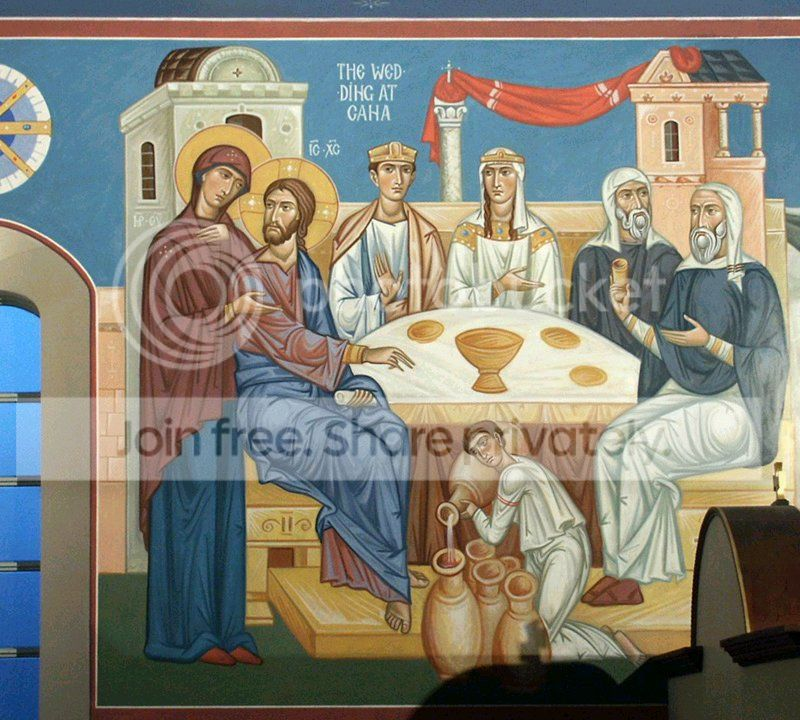
\includegraphics[width=.25\textwidth]{weddingatcannanicon.jpg}
\end{wrapfigure}

The mission of Christ and Mary is to reverse the effects of the Fall and restore the creation to its original perfect state when the Logos and Sophia brought it forth (Proverbs 8 22:31\footnote{\url{http://www.biblegateway.com/passage/?search=Proverbs+8&version=NKJV}}). Each of the seven miracles of St. John's Gospel corresponds to the reverse day of Genesis and restores to creation the grace bestowed by that day's miracle. The seven sacraments of the Church are based on the magic of evoking these miracles.

What I intend to show is that the last gospel is in fact an initiatic text, and that the seven miracles are intended to be a practical esoteric school which corresponds with the other western Traditions. As far as I know, it was the Catholic Hermeticist Valentin Tomberg\footnote{\url{https://en.wikipedia.org/wiki/Valentin_Tomberg}} who first elucidated this esoteric school in his last book, \textit{Lazurus Come Forth!}\footnote{\url{http://www.amazon.com/Lazarus-Come-Forth-Valentin-Tomberg/dp/1584200405}}. My spiritual practice and this essay owes much to it.

By applying the lessons of the seven miracles we spiritually grow, with the first miracle developing the faculties needed to master the latter ones. Like learning any set of skills that build on each other, you do not completely master a subject before progressing to the next. It can be compared to building a pyramid; laying down two bricks at the foundation allows you to place a brick on the second level; laying down three bricks on the first level allows you to build two on the second level and one on the third, etc. One simultaneously works on all levels which one can, always coming back to the basics as they are the foundation on which all the other levels depend.

Putting too much effort into the higher levels before one has prepared the foundation can be counter productive. For example, attempting to master the fifth miracle of walking on water (i.e. to make the will effortlessly immune to desire) by engaging in ascetic practices will likely fail if one hasn't become competent in the four preceding miracles, creating a large shadow which blocks the power from the lower chakras rather than putting their power at the disposal of the higher self.

This is like taking a brick and trying to suspend it five layers above the ground all by itself; it's just going to fall to the ground with no foundation under it. The capstone of the pyramid is the alchemic marriage; the spiritualization of matter; attaining the Resurrection Body, the fruit of the raising of Lazarus.

Each miracle will be listed, followed by the corresponding miracle of Genesis and sacrament, followed by some commentary.

\paragraph{The Turning of Water into Wine at the Wedding}


\emph{The union of God and His creation on the hallowing of the day of rest of the seventh day, i.e. the marriage of Heaven and Earth -- The Sacrament of Marriage}

Evokes the joyful celebration of God's union to His creation, the way wine at its best induces that state of ease and enjoyment which is proper to a joyous occasion. This corresponds to that other Christian esoteric school, the Tarot, which starts by teaching the same state with The Juggler/Magician card, who to successfully keep all the balls in the air must enter into the same lucid care free state of conscious. If he tries too hard to focus on the task or any individual ball he will drop them; to succeed he must stop trying and allow his awareness to expand past the individual objects he juggles.

Likewise, to be spiritually fruitful we need to change our everyday water (i.e. the mind which reflects objects) into the playful ease of wine (lucid experience, what psychologist have rediscovered as `flow\footnote{\url{http://en.wikipedia.org/wiki/Flow_\%28psychology\%29}}'). This creates the state of `concentration without effort' in which your work becomes married to heaven.

Specifically, when one is in the state of flow of the Juggler or the Wedding Guest, one is so focused on the joyous experience of the moment that everything else disappears, including the sense of one's own self. With the ego empty, inspiration is able to both emerge from the deeper levels of the self which are normally entombed by the ego, and to pour into us from above. Most people are like block(head)s into which nothing can be poured; it's only when we cultivate empty space that we become like a glass in which power from heaven can be poured.

Cultivating this state purifies the root chakra (and correspondingly all the odd/mental chakras) which governs instinct, removing the fear and anxiety which blocks it so that kundalini can begin to spiral heavenward up the spine and nourish the other centers of the soul.

Besides a progressive freeing from anxiety, the fruit of learning this lesson is mystical experience, as one enters into a state where one from time to time feels the presence of God.

\paragraph{The Healing of the Nobleman's Son}


\emph{The bringing forth of man and animals, each according to their kind on the sixth day -- The Sacrament of Baptism}

According to Tomberg, this healing was accomplished by bringing the son out of horizontal hereditary with his earthly father, and restoring him to resonance with the original archetype of his perfect heavenly Father. Likewise, this miracle brings us out of fallen horizontal hereditary and reestablishes our vertical hereditary to the spiritual archetype we emanated from, the image of God; the death to the sins of the world and spiritual rebirth of the baptismal waters.

One can note that Shamanic totemic magic is based on this principle of establishing an alliance with the perfect animal spirits in heaven so as to be drawn toward their virtues. This type of magic is well and alive in the employment of sport team mascots.

Reestablishing the vertical connection will result in the fruit of Gnosis, which is merely a mystical experience revealing itself to consciousness. When we live in the vertical that which is above reveals itself to us below. It's worth noting that the second card of the Tarot, the High Priestess, is the card which teaches the principles of the gnostic sense.

\paragraph{The Healing of the Paralytic}


\emph{The restoring of ensouled movement, in all directions; height, depth, and breadth; of the birds of the air and the fish of the sea on the fifth day -- The Sacrament of Penance}

``Go forth and sin no more.'' The Paralytic's condition was due to his sin, as evidenced by the Master's words after he had been healed. Sin enslaves and takes away our freedom, especially when we try to hide it within ourselves. The Persian branch of the Aryan tradition held that the greatest value was truth, and therefore the greatest sin one could commit was to lie. One could argue then that the gravest sin is to try and deny our own sins and hide them from ourselves. God will forgive us all our sins, on the prerequisite that we fully acknowledge them.

There's a lot I could say about this, as it relates directly to my vocation as a healer and massage therapist. People have all types of things they don't like about themselves, and usually they try to keep them from fully entering their consciousness. For example, they might detest one of their coworkers and want to give them a well deserved punch to the face. But if they did that they'd lose their job, plus they like to think of themselves as a good person, and good people don't get angry and violent, so they repress the impulse. On the physical level this produces nervous disorder\footnote{\url{http://en.wikipedia.org/wiki/John_E._Sarno}}; the subconscious prevents an unpleasant emotion or thought from reaching consciousness or the motor nerves, which results in the buried signal being held as an electric charge in the body, tightening the surrounding muscles.

Often when I work on someone I can feel the stuck emotion which is tightening the muscles. To treat them I allow the blocked emotion in the psyche and nerves to flow again, and the muscle goes back to normal, restoring ease of movement. Confession, when done right, allows people to acknowledge emotions they'd otherwise keep bottled up, thus healing them. This process purifies the second chakra which governs emotion (and correspondingly the other even emotional chakras), which is blocked by guilt.

The fruit of learning the third lesson is magic, which is simply the execution of that which is revealed by gnosis. Mysticism bears fruit by revealing itself as gnosis to consciousness, and gnosis bears fruit by becoming magic and flowing out into the world.

Continuing the correspondence to the tarot, the third card of the Tarot, the Empress, is the card that teaches sacred magic. The Empress holds a shield with an eagle on it. This is the aim of sacred magic, to defend the freedom (the eagle) of all ensouled beings, the movement through the heights, breadth, and depth which is taken away by retained sin.

\paragraph{Caution and Conclusion}


I will caution you that there's a reason the full extent of most people's emotions are sealed. If their full force were made manifest the world would become a very brutal place. As one of my shamanic instructors warned us, in traditional societies no parent wants their child to become a shaman, because it's very poor life insurance. Not all magic is sacred, and the soul is fragmented into both good and evil. Both come flowing out and manifesting themselves as the Work restores movement to the soul. I have had multiple people end up hospitalized after my heart cursed them, directing uncontrolled but sustained hatred their way. For example, the day I began unsealing my emotions toward my stepmother, she, who had been in robust health (my family follows my lead in eating paleo), ended up being hospitalized with intense pains whose cause could not be pinpointed.

This is why the two previous steps come first. Without them the unsealing of the soul's power would result in the Luciferian raising up of our arbitrary personal will and the uncontrolled releasing of demonic sorcery from the subconscious. In Traditional Orders this was guarded against by grades of initiation, to make sure the initiate was spiritually mature enough to face the next step, and the whole process was overseen by experienced masters. In the Kali Yuga it is very difficult to find such an Order, so the dangers are increased.

The Christian path has always been Purification, Illumination, and Union, the fruits of which are Mysticism, Gnosis, and Magic. In alchemy these are accomplished through `The work in black', `The work in white', and `The work in red' of lead, mercury, and sulfur; in the Tarot they are taught by the first three cards of `The Juggler', `The High Priestess', and `The Empress'; and in the Gospel of St. John the keys to realizing the work are contained in the first three miracles. As Gornahoor has pointed out, there is unity underlying the western tradition, and one can find all the essential esoteric elements needed for the Work hiding in plain sight within Christianity, which is the most accessible to those of us of the west.

Part 2 will continue with the remaining miracles. Before that will be an article expanding on the first two miracles; specifically how one can cultivate the mystic's 'emptiness' by contemplating and linking ones breath to the vertical originating archetype of God's breath which brought forth the Void and Sophia.


\flrightit{Posted on 2014-03-12 by Caleb}

\begin{center}* * *\end{center}

\begin{footnotesize}
\begin{sffamily}
\texttt{francismercuri on 2014-03-12 at 01:03 said:}

Thank you--this is most excellent. It happens to have appeared here in quite a timely fashion, as currently this evening my readings and note taking have involved Tomberg's discussion of ``The Chariot'' in his ``Meditations'', where he also addresses these very ``Seven archetypal miracles'', and their correspondence with the ``Seven `I Am'' statements of Christ. His ``departure point'' in that meditation, is the account of Christ's temptation in the wilderness, which also was the RC Rite Gospel reading for this past, first Sunday of Lent. Looking forward to your next installments.

\hfill

\texttt{scardanelli on 2014-03-12 at 09:44 said:}

Indeed... thank you for this Caleb. I have read Lazarus, Come Forth! previously, but for whatever reason, didn't make the connection between the seven miracles and the first seven arcana of the Tarot. It certainly opens up new areas to explore.

\hfill

\texttt{Frater M on 2014-03-12 at 13:40 said:}

As a handy reference, here follows the miracles/''I am'' statement pairings as given by Tomberg in his meditation on The Chariot. All chapters/verses refer to the Gospel of John:

1. Wedding of Cana (2)/''I am the true vine (15:1)\\ 2. Healing the noble's son (4:46)/''I am the Way, Truth, and Life'' (14:6)\\ 3. Pool of Bethesda (5:2)/''I am the door/gate'' (10:9)\\ 4. Feeding of 5000/multiplication of loaves (6)/''I am the bread of Life'' (6:35)\\ 5. Walking on water (6)/''I am the good shepherd'' (10:11)\\ 6. Healing the man born blind (9)/''I am the light of the world'' (8:12)\\ 7. Raising Lazarus (11)/''I am the resurrection and the life'' (14.6)

\hfill

\texttt{patriciakay3 on 2014-03-15 at 13:21 said:}

Thanks so much! I look forward to Part 2... it's very helpful material.

\hfill

\texttt{skeleton cave on 2019-03-19 at 11:43 said:}

That icon is taken at St. Seraphim's Orthodox Cathedral in Dallas, TX.

\hfill

\texttt{Tannheuser on 2022-03-31 at 14:46 said:}

I suppose the subsequent sections discussed never ended up being published? It's too bad -- these reflections are are a valuable supplement to Lazarus, Come Forth.

\end{sffamily}
\end{footnotesize}

